\chapter{Long-run Attacks}
\label{chap:towards_a_realistic_attack}

Until now, we considered the attacker dealing with single-action captures. In practice, an attacker might record possibly many different actions within one single, longer capture (because he cannot a priori know when each action starts and stops): we name this \textit{long-run} captures. This scenario extents to cases where a targeted victim stays for a while close-by to the attacker such as in an office. In this chapter, we test our attack on long-run captures. In addition, we discuss and address different challenges emerging from this setting: How to distinguish noise from actual actions, how to cut the traffic such that we do not miss the beginning or the end of an action. 

This section is structured as follows: First, we describe the experiment on long-run captures. Then, we explain the attack methodology. Finally, we present the results.

\section{Experiment Description}
In this chapter, all the experiments are done with the Huawei-Watch pair on 50 different actions: 33 openings and 17 in-app actions (see Sec.~\ref{sec:application opening identification} and Sec.~\ref{sec:in-App}) . We use the same setup as in Sec.~\ref{sec:data_generation} and extended our automation system by 200 LoC on the Central Controller to support long-run capture (see Sec.~\ref{sec:data_generation}). In our implementation, the automation system has three simulation modes: 

\begin{enumerate}
    \item \textbf{Deterministic inter-action launching}: The time in-between two consecutive actions launched on the smartwatch is deterministic 
    \item \textbf{Uniform inter-action launching}: The time in-between two consecutive actions launched on the smartwatch is randomly uniformly distributed
    \item \textbf{Interaction pattern inter-action launching}: The time in-between two consecutive actions launched on the smartwatch follows a specific user interaction pattern.
\end{enumerate}

We used the two first modes exclusively for training and validation, and the last mode exclusively for testing. In the two first modes, we arbitrarily set the waiting time mean of two consecutive actions to 50 seconds. For the third mode, we adjust the waiting time to follow the daily user interaction pattern based on the work of Liu, et al \cite{10.1145/3081333.3081351}. Fig.~\ref{fig:user_interaction_pattern} compares the daily user pattern interaction from the original paper and our simulation. Due to technical reasons, instead of considering portion of one hour, we considered slots of 20 minutes, and performed three times the experiment to have a total of 24 hours capture; which corresponds to 2.2 GB.





\begin{figure}[H]
\centering
\begin{subfigure}{.5\textwidth}
  \centering
  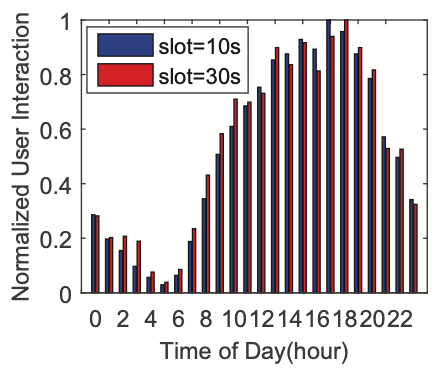
\includegraphics[width=0.92\textwidth]{figures/user interaction.png}
\end{subfigure}%
\begin{subfigure}{.5\textwidth}
  \centering
  \includegraphics[width=1.05\textwidth]{figures/plots/reproduced_user_interaction_level.png}
\end{subfigure}
\caption{\textbf{Left:} Daily user interaction pattern (from Liu, et. al). \textbf{Right:} Reproduced user interaction level on performed action triggered}
\label{fig:user_interaction_pattern}
\end{figure}
\\
 

Moreover, Liu et. al, reported that some applications are more likely to be triggered. Therefore, we give higher prior launching probability for actions belonging to the popular apps described by Liu et. al in Fig.~\ref{fig:popular apps}. However, due to the lack of information about how more frequent these applications are, we arbitrarily set their prior probability to be 1.5x higher than other apps. The rest of the applications are launched with equiprobability.


\begin{figure}[H]
 \centering
 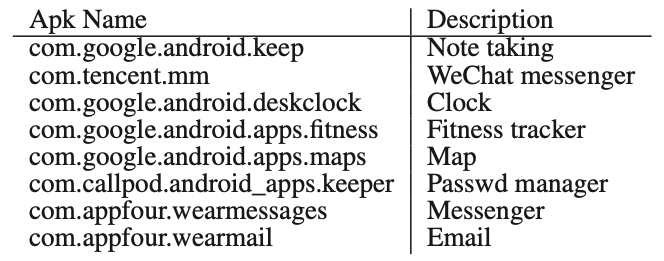
\includegraphics[width=0.5\textwidth]{figures/popular apps.png}
 \caption{Popular applications on smartwatches more likely to be triggered by a user (from Liu, et.  al~\cite{10.1145/3081333.3081351}).}
 \label{fig:popular apps}
\end{figure}


\section{Methodology}
\label{sec:longrun methodology}
Three building blocks composed the attack. First, the long-run capture is processed by a Sequence Splitter, whose job is to output chunks containing traffic of one single action performed on the smartwatch. A classifier then takes these chunks as input and outputs the probability of each chunk to belong to a specific class. Finally, the Decision Maker gives the final output from the vector probability. In all the modules, mechanisms are deployed to prevent noise to be wrongly classified as actions. Fig. \ref{fig:longrun methodology} gives an overview of the attack on a long-run capture.


\begin{figure}[H]
 \centering
 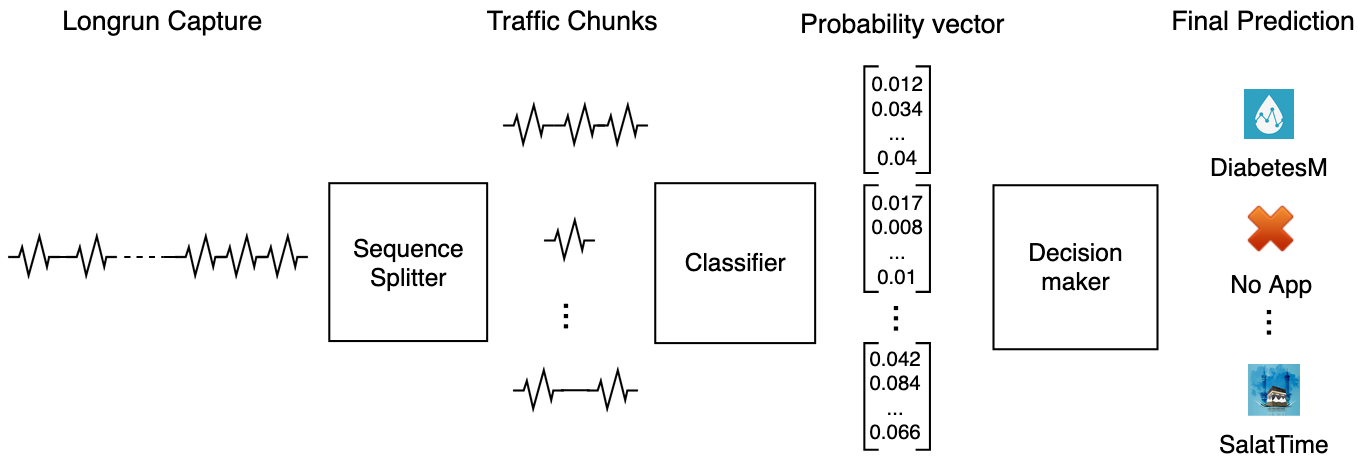
\includegraphics[width=0.98\textwidth]{figures/longrun overview 2.png}
 \caption{Overview of the attack on long-run captures.}
 \label{fig:longrun methodology}
\end{figure}

\paragraph{Sequence Splitter.} To process the long-run capture, the Sequence Splitter first identifies the points where an action might start (i.e. starting points). These starting points are found by moving a Sliding Window with length T seconds on the long-run capture. A point is considered as a starting point if the sum of packets length within the Window is more than N bytes. We choose N=200 bytes since action's traffic must contain more than 200 bytes (to pass the filter we designed for single-action capture, see Sec.~\ref{subsec:Filtering out Application}). We choose T=15 seconds based on training on the two first simulation modes and by intuition on the duration length of the traffic generated by a performed action\footnote{It is interesting to note that both parameters have different impacts on precision and recall for the two different action types (i.e. openings and in-app action)}. Then, from each starting point we determine the termination point, where the potential action might stop. A termination point is found if for a period of more than T seconds we do not receive any packets of length more than N bytes. Here, we choose N=46 because we consider packets with length smaller than 46 as noise (see Sec.~\ref{sec:model selection}), and T=10 in the same way as for the starting points. We note that the Sequence Splitter is designed such that an attacker does not need to wait the end of the long-run capture to make a prediction, and can process the long-run capture in real-time.


\paragraph{Classifier.} We build the same classifier as the one for the attack on single-action capture (see Sec.~\ref{sec:model selection}), yet with the following changes: we added one more class on top of the 50 targeted classes. This class serves as a filter to flag noise not related to targeted action. During our experiment, we realised that sometimes applications also generate traffic at closing, which is less fingerprintable so we decided to include these types of traffic to the extra class. Also, to attenuate the effect of ageing, we reused the dataset which spanned over 33 days (see Sec.~\ref{sec:eval over time}). Finally, the classifier does not output directly the prediction, but a probability vector representing its confidence about a particular class.

\paragraph{Decision Maker.} The Decision Maker takes has input the probability vector and outputs the majority voting only if the highest value in the vector is above a specific threshold. Otherwise a flag No App is outputted. The threshold then represents the sensitivity to make a prediction and is adapted to the attacker's requirement. A lower threshold will result in a  higher sensitivity (higher recall score but lower precision score) while a higher threshold in a lower sensitivity (a lower recall score but a higher precision score).





\newpage


\section{Attack on Long-run Evaluation}
If we do not consider prior probabilities and application removed, we know from Sec.~\ref{chapter summary}, that the higher accuracy we can have is 88.5\% (+/-2.6\%). In this section, we want to see how close we are from this experimentally discovered upper bound. However, accuracy is not suitable anymore; since now, a prediction might fail, not only because of misclassification, but also by trying to classify traffic that is not related to any action, or by simply missing an action. Therefore, we need to redefine the values TP, FP, and FN (introduced in Sec.~\ref{sec:background evaluation}) to a higher point of view, by considering not TP, FP and TN at a class level but at a prediction level:

\begin{itemize}
    \item \textbf{True Positive (TP):} Number of \textbf{correct predictions}. The Prediction at a particular time match the action performed on the watch at this time.

    \item \textbf{False Positive (FP):} Number of \textbf{wrong predictions}. The prediction at a particular time does not match the action performed on the watch at this time or there is no performed action at this time.

    \item \textbf{False Negative (FN):} Number of \textbf{missed performed actions}. The action performed on the watch at a particular time does not match any prediction at this time. 
\end{itemize}


Precision and recall are then computed the same way as in Sec.~\ref{sec:background evaluation}. Now, precision represents the fraction of time a prediction is correct regardless of whether there is no associated action at that time or the action is not the one predicted. Whereas Recall represents the fraction of time actions performed on the smartwatch are corrected classified.
\\

We will first test the attack on different degrees of sensitivity to know at which precision - recall range an attacker might operate. To this end, we increase the threshold value of the Decision Maker from 0 to 1 and monitor the precision, recall and F1 score. The plot is shown in Fig.~\ref{fig:longrun_p_r_f1_threshold}. 





\begin{figure}[ht]
 \centering
 \includegraphics[width=0.50\textwidth]{figures/plots/longrun_p_r_f1_threshold.png}
 \caption{Precision, Recall and F1 score for different Decision Maker's threshold.}
  \label{fig:longrun_p_r_f1_threshold}
\end{figure}





 The maximum recall score with the highest precision score is obtained by setting the Decision Maker's threshold at 0.1 and gives \textbf{83.5\%} recall score for 74.9\% precision score. On the contrary, a maximum precision score is reached at a threshold of 0.8 with a score of \textbf{100\%}. However the recall score at this threshold is only 23.5\%. With this setting, out of the 50 actions only 26 actions are retrieved, more specifically, none of the in-app actions are retrieved (but apps like ChinaDaily, DiabetesM or Spotify are retrieved at opening). Since we do not favor either precision nor recall, we will continue our analysis at which the best F1 score is achieved: \textbf{83.9\%}, for a precision score of 88.7\% and a recall score of 79.6\%. We summarize these results in  Tab.~\ref{tab:p_r_f_thre}.
 \\
 
\begin{table}[ht]
\centering
\begin{tabular}{lrrr}
\toprule
threshold  &  precision&    recall &        F1 \\
\midrule
0.10      &         74.9\% &  \textbf{83.5\%} &  79\% \\
0.80      &         \textbf{100.0\%} &  23.5\% &  38\% \\
0.25      &         88.7\% &  79.6\% &  \textbf{83.9\%} \\
\bottomrule
\end{tabular}
\caption{Precision, Recall and F1 score for different Decision Maker's threshold.}
\label{tab:p_r_f_thre}
\end{table}
\\
 
 We focus our attention to the performance of the attack according to the time of the day. Fig.~\ref{fig:towards_by_slots} shows the number of TP, FP and FN at each time slot. We can clearly identify the pattern of Fig.~\ref{fig:user_interaction_pattern}. We also see how the number of wrong predictions and missed prediction scales with the slots. However, we notice that slots having a low inter-action level achieve a lower prediction-recall score (the proportion between TP and FP and FN in these slots is smaller). Indeed, the 6 worst time slots in terms of F1 scores all belong to slot 0 to 6. We notice that in these slots, the noise compared to the actual information is bigger letting more room for an attacker to confuse noise as actual action. Therefore, an attacker might want to adapt the sensitivity of its model according to the time of the day. 
 
 
\begin{figure}[ht]
 \centering
 \includegraphics[width=0.70\textwidth]{figures/plots/towards_1tpfpfn.png}
 \caption{Number for TP FP and FN by slots.}
  \label{fig:towards_by_slots}
\end{figure}
 \\
 

 
 
 
 

  
We know that, due to close similarities, in-app actions might be less reliably fingerprinted than opening actions (see Sec.~\ref{sec:in-App}). To see that it applies also for long-run captures, we plot the precision-recall difference separated by these two kinds of actions in Fig~\ref{towards_action_types_pr}. We observe that indeed, in-app actions hurt the overall recall and precision score more than opening actions. However, we can also use in-app actions to target application. Fig.~\ref{fig:When only application are targeted} shows the adapted precision recall when applications alone are targeted. In that case, the overall F1 score is increased by 2\%, and on the specific in-app action type, we report an increase of 17\% for the recall and 14.3\% for the precision. These results confirmed that in many cases, misclassification of in-app actions was at the origin of the prediction's failure. To remove any ambiguity, we clarify that in the rest of this thesis we continue to identify specific in-app actions, and not group them by application.


\begin{figure}[H]
\centering
\begin{subfigure}{.5\textwidth}
  \centering
  \includegraphics[width=0.9\textwidth]{figures/plots/towards_action_types_inApp_targeted_action types_pr.png}
  \caption{When all actions and applications are targeted}
  \label{towards_action_types_pr}
\end{subfigure}%
\begin{subfigure}{.5\textwidth}
  \centering
  \includegraphics[width=0.9\textwidth]{figures/plots/towards_action_types_App_targeted_action types_pr.png}
  \caption{When only applications are targeted}
  \label{fig:When only application are targeted}
\end{subfigure}
 \caption{Precision and recall for different kind of actions.}
  \label{fig:towards_action_types_pr}
\end{figure}


 

 We finish our analysis by exploring which actions are more fingerprintable than others, as we did in Sec.~\ref{chapter summary}, but in the context of long-run captures. We expect to see significant changes since noise can be misclassified as a class, and the Sequence Splitter might wrongly cut the traffic. First we note that seven actions have zero F1 score. We identify several reasons for that. First, due to prior probabilities (actions more/less likely to be triggered due to popularity, see Fig.~\ref{fig:popular apps}), the specific action was not triggered enough to show some results. Second, some of these seven actions had already low F1 score. Third, the sensitivity of the Descision Maker is too low to recall any instances of these actions. On the contrary, we see that seven apps achieved 100\% F1 scores, whereas we only had one app achieving such score. Here again, this might come from a lack in the number of realisations performed to show more accurate results. We also note that few actions have high F1 score on single-action capture but poor score on long-run captures (such as the native app Weather). Even though sensitivity of the Decision Maker can explain part of that, we point out that a particular application might generate traffic similar to noise. Since our classifier also classify noise (as opposed to the classifier of single-action capture), instances of this application might be wrongly classified as noise and thus explaining the F1 score gap between single-action and long-run capture on particular applications. 
 \\
 
 We give a sample of results in Tab.~\ref{tab:rank summarize longrun} taken from the overall ranking based on F1 score for long-run captures (see Tab.~\ref{tab:attack ranking longrun}). The column count is the number of times a specific action was performed on the smartwatch during the long-run capture. For better comparison, with the experiment on single-action capture, we extracted the same samples as in Tab.~\ref{tab:rank summarize}, and show in column F1 sa. the F1 score of that action on single-action captures.
 \\
 
\begin{table}[H]
\centering
 \begin{tabular}{lllllll} 
 \toprule
 application name & action & F1 sa. & F1 & precision & recall & count \\ [0.5ex] 
 \midrule
FoursquareCityGuide & coffee &   30.78  &   33.33 &      50.00 &   25.00 &      4 \\
DiabetesM & addInsulin       &  74.19  &   66.67 &     100.00 &   50.00 &      2 \\
Shazam & open                &  95.08  &   93.33 &     100.00 &   87.50 &     16 \\
Lifesum & addFood            &  99.51  &   88.89 &     100.00 &   80.00 &      5 \\
DiabetesM & open             &  100.00  &   97.96 &     100.00 &   96.00 &     25 \\
 \bottomrule
\end{tabular}
\caption{Sample extracted from the overall ranking on long-run capture by class according to their F1 score (see Tab.~\ref{tab:attack ranking longrun}). Also shown: the F1 score on single-action capture (column F1 sa.) extracted from the same samples in Tab.~\ref{tab:rank summarize longrun}}
    \label{tab:rank summarize longrun}
\end{table}

\newpage

Throughout our evaluation, we targeted many applications. However, most attackers might be interested in targeting one single application with specific requirement on precision and recall. So the question is how would such attacker proceed? One possible way is to follow the exact same steps explained in this section but instead of having 50 targeted classes plus one noise class, the attacker would have only two classes: one target class and one noise class. To fix the threshold of the Decision Maker (if we suppose that the attacker is interested $\beta$ times more in recall than in precision), the attacker will maximise the $F_\beta$ score instead of the $F_1$ score. This kind of attacker would certainly achieve much better performance on this specific targeted action than the results we provided here.
